\documentclass[conference]{IEEEtran}
\IEEEoverridecommandlockouts
\usepackage{cite}
\usepackage{amsmath,amssymb}
\usepackage{graphicx}
\usepackage{booktabs}
\usepackage{array}
\usepackage{tabularx}
\usepackage{xcolor}
\usepackage{tikz}
\usetikzlibrary{positioning,arrows.meta,fit,backgrounds,calc,shapes.misc}
\usepackage[hidelinks]{hyperref}

\definecolor{maroon}{RGB}{80,0,0}
\definecolor{maroonsoft}{RGB}{244,232,232}
\definecolor{sun}{RGB}{217,150,43}
\definecolor{ink2}{RGB}{80,80,80}
\definecolor{ctrl}{RGB}{23,128,138}
\definecolor{cellbg}{RGB}{243,241,239}
\newcolumntype{L}[1]{>{\raggedright\arraybackslash}p{#1}}
\newcolumntype{Y}{>{\raggedright\arraybackslash}X}

\begin{document}

\title{Supplying Inflexible AI Data Centers with Hourly Clean Energy: A Smart-Grid Review of Internal and External Flexibility}

\author{\IEEEauthorblockN{[Author Name]\IEEEauthorrefmark{1} and [Advisor Name]\IEEEauthorrefmark{1}}
\IEEEauthorblockA{\IEEEauthorrefmark{1}Department of Electrical and Computer Engineering, Texas A\&M University, College Station, TX, USA\\
Email: [email]}}

\maketitle

\begin{abstract}
Artificial-intelligence (AI) data centers are large, nearly constant loads that must be supplied reliably and, increasingly, with clean energy matched hour by hour. This paper reviews how the literature reconciles these requirements. From a structured search of 1{,}365 records, 53 studies are analyzed across three research streams---the internal flexibility of data centers, clean-energy matching for large consumers, and demand-side flexibility in the power system---and placed in the smart-grid context, as distinct from microgrid solutions. We propose a positioning model that classifies the literature by the source of flexibility and its purpose, and we compare supply options on reliability, hourly clean supply, cost and grid impact. Three findings emerge. Internal flexibility, the field's dominant assumption, is small for AI facilities: about 6\% of facility power is immediately curtailable. Hourly matching relies on procured generation and storage, whose requirements grow non-linearly above about 80\%, or on the buyer's own flexibility. Demand flexibility from other loads is substantial---7.1--29.9~GW of industrial potential in Saudi Arabia by 2030---yet it is procured only by system operators for system services. The intersection, contracting the flexibility of other grid loads to deliver hourly clean supply to an inflexible data center, is unexplored. We define it as External Energy Flexibility and derive a research agenda.
\end{abstract}

\begin{IEEEkeywords}
AI data centers, smart grid, demand response, aggregation, hourly matching, 24/7 carbon-free energy, energy storage, microgrids, review.
\end{IEEEkeywords}

\section{Introduction}
Data centers used about 415~TWh, or 1.5\% of global electricity, in 2024, and their consumption is projected to more than double to about 945~TWh by 2030, with AI the main driver~\cite{r40}. In the United States they used 4.4\% of electricity in 2023 and may reach 6.7--12\% by 2028~\cite{r1}; Saudi Arabia's national strategy targets about 1.5~GW of data-center capacity by 2030~\cite{r52}, and a 1.5-GW AI campus announced for NEOM is described as net-zero yet will initially draw power from thermal plants~\cite{r53}. AI facilities draw power that is high and nearly constant: in a 155{,}410-GPU production trace, immediately curtailable load averaged only about 6\% of median facility power~\cite{r26}. Grid connections for such loads can take more than five years, driving some operators toward microgrids with dedicated generation~\cite{r28}.

Three requirements frame how these loads should be supplied. They must be \emph{reliable}, with availability designed to tier standards~\cite{r41}. They must be \emph{clean in a credible way}: annual matching of renewable purchases to consumption overstates real mitigation~\cite{r12}, hourly (24/7) matching is needed for system-level reductions~\cite{r10,r11}, and carbon-accounting rules are being revised toward hourly matching~\cite{r50}. And they must be \emph{affordable}, without adding to already congested grids~\cite{r27,r28}.

Existing reviews cover parts of this problem: data-center demand response~\cite{r3}, demand response and smart grids~\cite{r17,r57}, aggregators~\cite{r59}, renewable-storage sizing~\cite{r30} and data-center energy estimates~\cite{r29}. None examines how the three bodies of work combine to supply an \emph{inflexible} AI data center. This paper makes three contributions: (i) a structured review of 53 studies across three research streams, framed by smart-grid and microgrid concepts; (ii) a positioning model of the literature and a comparison of supply options against the three requirements and grid impact; and (iii) the identification of an unexplored option, External Energy Flexibility, with a research agenda. Section~II describes the method, Section~III the background, Section~IV the three streams, Section~V the synthesis, and Section~VI concludes.

\section{Review Method}
Searches were run in November 2026 in Crossref, which indexes IEEE, Elsevier, Springer, ACM, IOP and MDPI publications, and in IEEE Xplore, Semantic Scholar and arXiv, for publications from 2010 to 2026 on seven themes (Fig.~\ref{fig:method}). Grey literature from the IEA, LBNL, KAPSARC, standards bodies and government agencies was added, as were earlier works found by backward citation tracking. Studies were included if they (i) addressed the supply or flexibility of data centers or other large loads; (ii) proposed or evaluated a means of hourly clean-energy matching; (iii) characterized demand-side flexibility or its procurement; or (iv) provided assessment methods or Saudi-specific evidence. Peer-reviewed work was preferred; preprints were kept only for recent evidence not yet in journals. Ten foundational smart-grid and microgrid references were added to frame the contribution. The field is recent: 25 of the 53 studies date from 2024--2026 (Fig.~\ref{fig:years}).

\begin{figure}[!t]
\centering
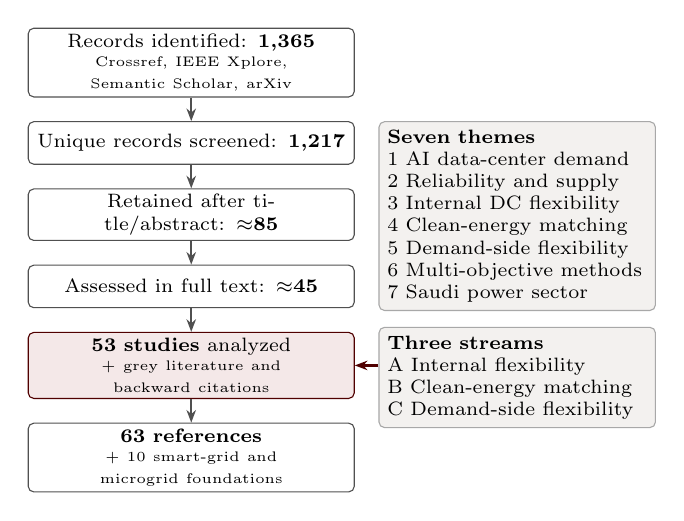
\begin{tikzpicture}[font=\scriptsize,
  box/.style={draw=ink2, rounded corners=2pt, fill=white, align=center, minimum height=5.4mm, inner sep=2pt},
  side/.style={draw=ink2!50, rounded corners=2pt, fill=cellbg, align=left, inner sep=3pt, text width=33mm},
  arr/.style={-{Stealth[length=1.6mm]}, draw=ink2, thick}]
\node[box, text width=40mm] (a) {Records identified: \textbf{1,365}\\[-1pt]{\tiny Crossref, IEEE Xplore, Semantic Scholar, arXiv}};
\node[box, text width=40mm, below=3mm of a] (b) {Unique records screened: \textbf{1,217}};
\node[box, text width=40mm, below=3mm of b] (c) {Retained after title/abstract: \textbf{$\approx$85}};
\node[box, text width=40mm, below=3mm of c] (d) {Assessed in full text: \textbf{$\approx$45}};
\node[box, text width=40mm, below=3mm of d, fill=maroonsoft, draw=maroon] (e) {\textbf{53 studies} analyzed\\[-1pt]{\tiny + grey literature and backward citations}};
\node[box, text width=40mm, below=3mm of e] (f) {\textbf{63 references}\\[-1pt]{\tiny + 10 smart-grid and microgrid foundations}};
\foreach \u/\v in {a/b,b/c,c/d,d/e,e/f} \draw[arr] (\u) -- (\v);
\node[side, right=3mm of b.north east, anchor=north west] (t) {\textbf{Seven themes}\\
1 AI data-center demand\\2 Reliability and supply\\3 Internal DC flexibility\\4 Clean-energy matching\\5 Demand-side flexibility\\6 Multi-objective methods\\7 Saudi power sector};
\node[side, below=2mm of t] (s) {\textbf{Three streams}\\
A Internal flexibility\\B Clean-energy matching\\C Demand-side flexibility};
\draw[arr, draw=maroon] (s.west |- e.east) -- (e.east);
\end{tikzpicture}
\caption{Review protocol, themes and the three research streams analyzed.}
\label{fig:method}
\end{figure}

\begin{figure}[!t]
\centering
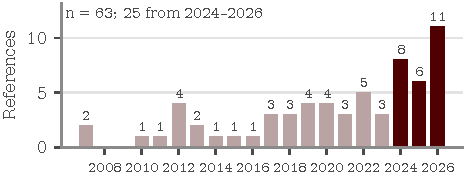
\includegraphics[width=\columnwidth]{fig_years.pdf}
\caption{References by publication year; 2024--2026 highlighted.}
\label{fig:years}
\end{figure}

\section{Background: Reliability and Supply Configurations}
\emph{Reliability.} The tier classification grades data-center configurations from Tier~1 to Tier~4, each step removing single points of failure~\cite{r41}. Uninterruptible power supplies (UPS) and generators ride through disturbances, and grid-interactive UPS can provide fast frequency response with full activation within about a second~\cite{r7}, but these assets are not designed to supply a facility for hours. Any supply option must therefore preserve availability at the point of supply, while large constant loads also burden system adequacy: connection queues delay new data centers by years~\cite{r28}, and capacity-expansion studies distinguish firm, flexible and interruptible data-center load~\cite{r27}.

\emph{Supply configurations.} Three configurations dominate. (1) \emph{Direct grid supply} inherits the grid's reliability and carbon intensity. (2) \emph{On-site or colocated renewables with storage}~\cite{r8,r22} is a sizing problem: batteries are sized to a loss-of-power-supply probability~\cite{r31} or traded against loss-of-load and loss-of-energy expectations~\cite{r32}, and a review finds empirical sizing tends to waste resources~\cite{r30}. Storage dominates cost as the renewable share rises: for an industrial consumer, required storage grows non-linearly beyond about 80\%~\cite{r15}; costs are falling~\cite{r43}, but the escalation near 100\% persists~\cite{r11,r15}. (3) \emph{Contracted renewables}, through corporate power purchase agreements (PPAs)~\cite{r42} and certificates, matched annually or hourly (Section~IV-B). Siting studies increasingly weight renewable potential~\cite{r34} and water stress~\cite{r35}.

\section{Three Research Streams}
\subsection{Internal Flexibility of Data Centers}
The established view is that data centers are flexible loads. Workload shifting with local generation avoided coincident-peak charges, saving up to 40\% of electricity costs under one coincident-peak tariff~\cite{r2}; peak shaving was formulated as joint control of delay-tolerant workloads and batteries~\cite{r6}; and demand response was co-optimized with server provisioning and procurement in a two-stage stochastic program~\cite{r5}. Reviews and load models organize spatial and temporal workload regulation~\cite{r3,r4}. For AI facilities, recent studies co-optimize workload scheduling with colocated renewables~\cite{r8}, embed deferrable AI load in capacity expansion~\cite{r24}, shift computation in time and space for 24/7 matching~\cite{r9}, and show that the value of flexibility depends on the host grid~\cite{r27}.

\emph{Common assumption and appraisal.} All of these draw flexibility from \emph{inside} the data center. Measured on an AI production trace, immediately curtailable load averages about 6.35\% of median facility power, and a share calibrated on mean values overstates dependable relief by 17\%, 25\% and 47\% for 1-, 4- and 24-hour events~\cite{r26}. Flexibility is also evaluated mainly for cost or grid services rather than for the data center's own clean supply, and rarely under reliability constraints.

\subsection{Clean-Energy Matching for Large Consumers}
\emph{Annual matching} procures renewable energy equal to annual consumption. Excluding certificate-based claims, 42\% of committed scope~2 reductions of companies with science-based targets would not result in real mitigation~\cite{r12}, and annual-average accounting can bias inventories by up to $\pm$35\%~\cite{r13}. Fig.~\ref{fig:mismatch} shows why for a constant load: energy is matched over the day, but not hour by hour. Capacity-expansion studies find that annually matched procurement has negligible emission benefits, whereas \emph{hourly} matching reduces system emissions at a premium that is small for 90--95\% but high for 100\% with solar, wind and batteries alone~\cite{r10,r11}.

\begin{figure}[!t]
\centering
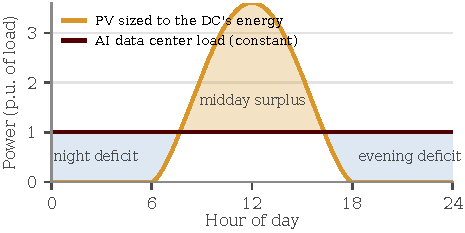
\includegraphics[width=\columnwidth]{fig_mismatch.pdf}
\caption{Illustrative day: PV sized to a constant load's energy leaves a midday surplus and night and evening deficits that hourly matching must bridge.}
\label{fig:mismatch}
\end{figure}

Hourly matching is achieved by three means: (i) portfolios of procured clean generators that reach a target hourly score at least cost~\cite{r16}; (ii) storage and firm resources, sized with risk-averse stochastic planning~\cite{r14} or combined with direct PPAs, where storage requirements grow non-linearly beyond about 80\%~\cite{r15}; and (iii) the buyer's \emph{own} flexibility~\cite{r9,r10}. Accounting rules frame these choices: the GHG Protocol requires location- and market-based scope~2 reporting~\cite{r49}, a 2025 consultation proposed hourly, deliverable matching~\cite{r50}, and granular certificates have been standardized~\cite{r51}. Average and marginal emission factors differ~\cite{r46,r47}; in Saudi Arabia the marginal generator largely does not change with load timing under the 2017 mix~\cite{r38}.

\emph{Common assumption and appraisal.} Hourly matching uses supply-side assets or the buyer's own load. Studies concentrate on the United States, Europe and Korea; none examines a single-buyer market or treats other consumers' flexibility as a procurable means of matching.

\subsection{Demand-Side Flexibility in the Power System}
Demand response combines incentive- and price-based programs, enabling technologies and measurement against customer baselines~\cite{r17}, and reliable baselines are a precondition for fair remuneration~\cite{r45}. Flexibility is procured by system operators directly or through aggregators~\cite{r18}. Industrial loads are characterized as resources: desalination plants can adjust power while meeting water demand~\cite{r20}, with flexibility intervals quantified by adaptive robust optimization~\cite{r19}, and aggregators can shift load toward solar hours~\cite{r21}; highly renewable grids need such flexibility together with policy change~\cite{r25}. Its value is not constant: as solar penetration rises, the market value of solar output falls~\cite{r44}, creating value for loads that absorb midday energy, while the value of a resource declines the more it is activated~\cite{r23,r27}. In Saudi Arabia, which targets 50\% renewable electricity by 2030 with solar the leading resource~\cite{r36,r37,r48}, the depth of the daily net-load ``duck curve'' is projected to triple from 2025 to 2030 and industrial demand-response potential is 7.1--29.9~GW, but the role of flexibility in the single-buyer market is undefined~\cite{r23}.

\emph{Common assumption and appraisal.} External flexibility is procured \emph{by the system operator} for \emph{system services}; the literature does not link it to a specific consumer's supply.

\subsection{Smart Grids and Microgrids}
The smart grid adds information, communication and control across the generation, transmission, distribution, customer, market, operations and service-provider domains so that resources in all of them can be coordinated~\cite{r54,r55}, with demand-side management and renewable integration among its central functions~\cite{r56,r57}. Aggregators and virtual power plants pool distributed resources~\cite{r58}, and their lasting value comes from economies of scale and scope~\cite{r59}; model predictive control is the established method for operating flexible loads such as buildings~\cite{r60}. A microgrid, by contrast, is a group of loads and resources within clear electrical boundaries that acts as one controllable entity and can island~\cite{r61,r62,r63}. On-site renewables with storage and off-grid data-center designs are microgrid solutions (Table~\ref{tab:sgmg}, Fig.~\ref{fig:model}).

\begin{table}[!t]
\caption{Smart Grid and Microgrid Compared}
\label{tab:sgmg}
\centering
\scriptsize
\begin{tabularx}{\columnwidth}{@{}L{14mm}YY@{}}
\toprule
Aspect & Smart grid & Microgrid \\
\midrule
Scope & Interconnected system, national or regional & One site within defined electrical boundaries \\
Coordination & Distributed: operator, aggregators, markets & One local controller \\
Grid relation & Relies on interconnection & Can island \\
Functions & Demand response, aggregation, metering, settlement & Local reliability, self-supply \\
DC example & Grid-interactive DC; contracted external flexibility & On-site PV and battery; off-grid campus \\
\bottomrule
\end{tabularx}
\end{table}

\begin{figure}[!t]
\centering
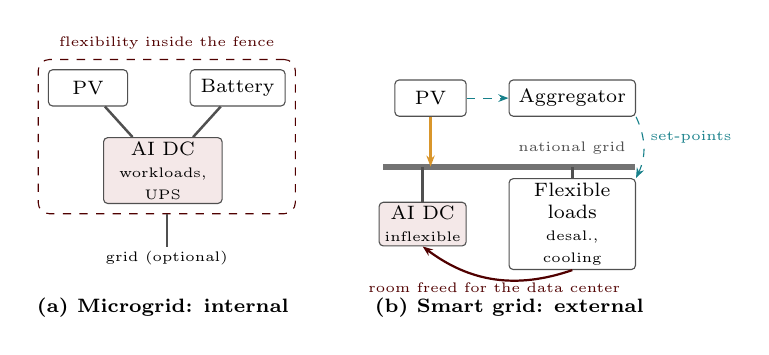
\begin{tikzpicture}[font=\scriptsize,
  dev/.style={draw=ink2, rounded corners=1.5pt, fill=white, align=center, inner sep=1.5pt, minimum height=4.6mm},
  pw/.style={draw=ink2, line width=.9pt},
  sol/.style={draw=sun, line width=.9pt, -{Stealth[length=1.4mm]}},
  info/.style={draw=ctrl, dashed, -{Stealth[length=1.3mm]}}]
% (a) internal flexibility: microgrid
\node[dev, fill=maroonsoft, text width=14mm] (dc1) at (0,0) {AI DC\\{\tiny workloads, UPS}};
\node[dev, text width=9mm] (pv1) at (-0.95,1.05) {PV};
\node[dev, text width=11mm] (bt1) at (0.95,1.05) {Battery};
\draw[pw] (pv1) -- (dc1); \draw[pw] (bt1) -- (dc1);
\begin{scope}[on background layer]
\node[draw=maroon, dashed, rounded corners=4pt, fit=(dc1)(pv1)(bt1), inner sep=3.5pt] (mg) {};
\end{scope}
\node[font=\tiny, text=maroon, anchor=south] at (mg.north) {flexibility inside the fence};
\draw[pw] (mg.south) -- ++(0,-0.42) node[below, inner sep=1pt] (g1) {\tiny grid (optional)};
\node[font=\scriptsize\bfseries, anchor=north] at (0,-1.5) {(a) Microgrid: internal};
% (b) external flexibility: smart grid
\begin{scope}[xshift=4.35cm]
\draw[draw=ink2!80, line width=2.2pt] (-1.55,0.05) -- (1.65,0.05);
\node[font=\tiny, text=ink2, anchor=south east] at (1.65,0.09) {national grid};
\node[dev, fill=maroonsoft, text width=10mm] (dc2) at (-1.05,-0.68) {AI DC\\{\tiny inflexible}};
\node[dev, text width=8mm] (pv2) at (-0.95,0.92) {PV};
\node[dev, text width=15mm] (ag) at (0.85,0.92) {Aggregator};
\node[dev, text width=15mm] (fl) at (0.85,-0.68) {Flexible loads\\{\tiny desal., cooling}};
\draw[pw] (dc2) -- (-1.05,0.05);
\draw[sol] (pv2) -- (-0.95,0.05);
\draw[pw] (fl) -- (0.85,0.05);
\draw[info] (ag.south east) to[bend left=25] (fl.north east);
\draw[info] (pv2.east) -- (ag.west);
\node[font=\tiny, text=ctrl, anchor=west] at (1.72,0.42) {set-points};
\draw[-{Stealth[length=1.3mm]}, draw=maroon, thick] (fl.south) to[bend left=28] node[below, font=\tiny, text=maroon, inner sep=1pt] {room freed for the data center} (dc2.south);
\node[font=\scriptsize\bfseries, anchor=north] at (0.05,-1.5) {(b) Smart grid: external};
\end{scope}
\end{tikzpicture}
\caption{Two ways to supply a data center with clean energy: (a) flexibility and storage inside a microgrid; (b) flexibility of other loads, coordinated through the smart grid.}
\label{fig:model}
\end{figure}

\section{Synthesis and Research Gap}
\subsection{Positioning Model}
Fig.~\ref{fig:position} classifies the literature by where flexibility comes from---inside the data center, the buyer's own supply assets, or other loads on the grid---and what it is used for. Every cell but one is occupied. Flexibility inside the data center serves both purposes but is small for AI loads~\cite{r26}; supply-side assets deliver hourly matching at escalating storage cost~\cite{r15}; and the flexibility of other loads serves only the system~\cite{r17,r18,r23}. No study uses the flexibility of other grid loads to provide a buyer's hourly clean supply.

\begin{figure*}[!t]
\centering
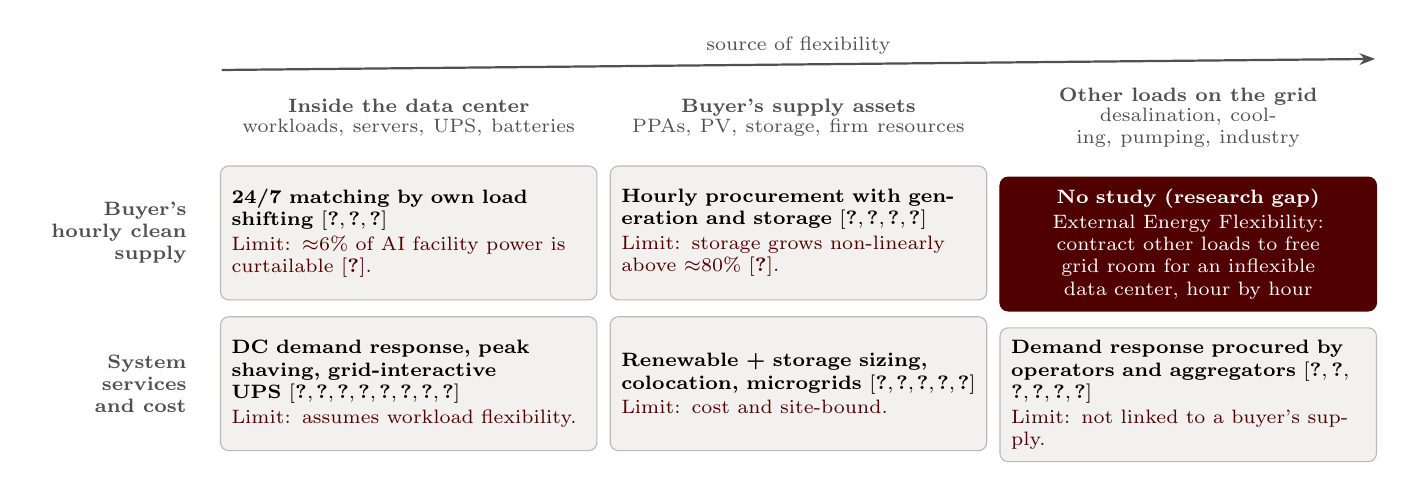
\begin{tikzpicture}[font=\scriptsize,
  cell/.style={draw=ink2!40, rounded corners=3pt, fill=cellbg, align=left, text width=45mm, minimum height=17mm, inner sep=4pt},
  gap/.style={draw=maroon, rounded corners=3pt, fill=maroon, text=white, align=center, text width=45mm, minimum height=17mm, inner sep=4pt},
  hd/.style={align=center, text width=45mm, font=\scriptsize\bfseries, text=ink2},
  rh/.style={align=right, text width=19mm, font=\scriptsize\bfseries, text=ink2}]
\node[hd] (h1) at (0,0) {Inside the data center\\[-1pt]{\normalfont workloads, servers, UPS, batteries}};
\node[hd] (h2) at (4.95,0) {Buyer's supply assets\\[-1pt]{\normalfont PPAs, PV, storage, firm resources}};
\node[hd] (h3) at (9.9,0) {Other loads on the grid\\[-1pt]{\normalfont desalination, cooling, pumping, industry}};
\node[cell, below=2.5mm of h1] (c11) {\textbf{24/7 matching by own load shifting}~\cite{r8,r9,r10}\\[1pt]\textcolor{maroon}{Limit: $\approx$6\% of AI facility power is curtailable~\cite{r26}.}};
\node[cell, below=2.5mm of h2] (c12) {\textbf{Hourly procurement with generation and storage}~\cite{r11,r14,r15,r16}\\[1pt]\textcolor{maroon}{Limit: storage grows non-linearly above $\approx$80\%~\cite{r15}.}};
\node[gap, below=2.5mm of h3] (c13) {\textbf{No study (research gap)}\\[1pt]External Energy Flexibility: contract other loads to free grid room for an inflexible data center, hour by hour};
\node[cell, below=2mm of c11] (c21) {\textbf{DC demand response, peak shaving, grid-interactive UPS}~\cite{r2,r3,r4,r5,r6,r7,r24,r27}\\[1pt]\textcolor{maroon}{Limit: assumes workload flexibility.}};
\node[cell, below=2mm of c12] (c22) {\textbf{Renewable + storage sizing, colocation, microgrids}~\cite{r22,r30,r31,r32,r33}\\[1pt]\textcolor{maroon}{Limit: cost and site-bound.}};
\node[cell, below=2mm of c13] (c23) {\textbf{Demand response procured by operators and aggregators}~\cite{r17,r18,r19,r20,r21,r23}\\[1pt]\textcolor{maroon}{Limit: not linked to a buyer's supply.}};
\node[rh, left=3mm of c11] {Buyer's hourly clean supply};
\node[rh, left=3mm of c21] {System services and cost};
\draw[-{Stealth[length=2mm]}, ink2, thick] ($(h1.north west)+(0,2.5mm)$) -- ($(h3.north east)+(0,2.5mm)$) node[midway, above, font=\scriptsize] {source of flexibility};
\end{tikzpicture}
\caption{Positioning model of the literature: source of flexibility (columns) against its purpose (rows). The only empty cell is the research gap addressed by External Energy Flexibility.}
\label{fig:position}
\end{figure*}

\subsection{Supply Options Against the Requirements}
Table~\ref{tab:options} compares the supply options. Direct grid supply and annual matching keep grid reliability but do not supply clean energy every hour~\cite{r12,r13}. Renewables with storage and hourly procurement portfolios do, but their storage needs escalate as matching approaches 100\%~\cite{r11,r15}. Internal flexibility is cheap but too small for constant AI loads~\cite{r26}.

\begin{table}[!t]
\caption{Supply Options for an Inflexible AI Data Center}
\label{tab:options}
\centering
\scriptsize
\setlength{\tabcolsep}{2.5pt}
\begin{tabularx}{\columnwidth}{@{}L{17mm}L{12mm}L{13mm}YL{12mm}@{}}
\toprule
Option & Reliability & Hourly clean & Cost at high shares & Grid room \\
\midrule
Grid only & grid & no & tariff only & adds load~\cite{r28} \\
Annual matching~\cite{r42} & grid & no~\cite{r12,r13} & low & as grid \\
RE + storage, microgrid~\cite{r30,r31,r32} & sized (LPSP) & yes & storage escalates above $\approx$80\%~\cite{r15} & reduced \\
Hourly portfolios~\cite{r14,r16} & grid-backed & yes & premium high near 100\%~\cite{r11} & system benefit~\cite{r10} \\
Internal DC flexibility~\cite{r2,r9} & unchanged & partial & low & some~\cite{r27} \\
\textbf{External flexibility (EEF)} & \textbf{grid} & \textbf{target} & \textbf{price of flexibility} & \textbf{to quantify} \\
\bottomrule
\end{tabularx}
\end{table}

\subsection{The Closest Studies}
Table~\ref{tab:closest} contrasts the closest studies. Those that achieve hourly matching rely on supply-side assets whose storage needs escalate~\cite{r11,r14,r15,r16} or on the data center's own flexibility~\cite{r8,r9}, which constant AI loads lack~\cite{r26}; studies of data-center flexibility take the system planner's view~\cite{r27}; and none is set in a single-buyer market. The closest work co-locates a \emph{flexible} data center with a reverse-osmosis plant, PV and storage behind one substation, uses data-center waste heat to preheat seawater, and cuts annualized cost by 86.5\%~\cite{r22}. The option proposed here differs in five respects: it targets an \emph{inflexible} data center; it draws on a \emph{portfolio of existing} grid-connected loads rather than one co-planned plant; the coupling is \emph{contractual} through the grid rather than physical; it targets hourly matching jointly with reliability and cost; and it is benchmarked against grid supply, renewables with storage and annual matching.

\begin{table*}[!t]
\caption{The Studies Closest to External Energy Flexibility}
\label{tab:closest}
\centering
\scriptsize
\begin{tabularx}{\textwidth}{@{}L{21mm}L{27mm}YL{38mm}L{15mm}L{27mm}@{}}
\toprule
Study & Data-center load & Means of matching or flexibility & Objective and method & Region & Gap relative to EEF \\
\midrule
Kwon et al.~\cite{r5} & Flexible (server provisioning) & Own servers; procured renewables, storage & Cost; two-stage stochastic & -- & Internal flexibility \\
Li et al.~\cite{r8} & Flexible AI DC & On-site renewables; market & Cost; energy management & U.S. & Internal, on-site \\
Riepin et al.~\cite{r9} & Flexible (spatio-temporal) & Renewables, storage, own shifting & 24/7 CFE cost; PyPSA & Europe & Needs DC flexibility \\
Xu et al.~\cite{r10} & Generic C\&I buyers & Clean generation, storage, own DR & System emissions, cost; GenX & Western U.S. & Buyer's own flexibility \\
Hwang et al.~\cite{r14} & Fixed DC, industrial & PV, wind, BESS, gas, certificates & Cost, shortfall risk; stochastic CVaR & Korea & Storage-intensive \\
Lee et al.~\cite{r15} & Fixed industrial & Direct PPA, market, storage & Procurement cost; MILP & Korea & Storage escalates $>$80\% \\
Ludkovski et al.~\cite{r16} & Fixed loads & Solar and wind PPA portfolio & Cost, chance-constrained CFE & U.S. (Texas) & Generation only \\
Yang et al.~\cite{r22} & Flexible DC & Co-located desalination, PV, storage & Annualized cost; stochastic MINLP & Arid coasts & Flexible DC; one plant \\
Khanal et al.~\cite{r27} & Firm/flexible/interruptible & DC's own shifting, curtailment & System cost; capacity expansion & PJM, Korea & Planner's view \\
\midrule
\textbf{EEF (gap)} & \textbf{Inflexible AI DC} & \textbf{Grid-injected PV; portfolio of external loads; contract} & \textbf{Hourly matching, reliability, cost} & \textbf{Single-buyer} & -- \\
\bottomrule
\end{tabularx}
\end{table*}

\subsection{Research Gap and the EEF Concept}
No study was found that (i) treats a constant-load AI data center as inflexible; (ii) pairs it with grid-injected PV sized to its annual consumption; and (iii) achieves hourly clean supply by contracting the flexibility of external loads already on the grid, evaluated jointly on reliability, cost and sustainability against the established options. We call this option \emph{External Energy Flexibility} (EEF). The data center stays fully grid-supplied, so its reliability is the grid's; its PV output is sold to the grid; and contracted flexible loads elsewhere use that output at midday and step back at night by as much as the data center uses, freeing grid room for it hour by hour (Fig.~\ref{fig:model}b). EEF is a smart-grid service rather than a microgrid: it relies on aggregation, metering and scheduling across the customer, service-provider, operations and market domains~\cite{r54}, and the scale economies of aggregation~\cite{r59} imply a minimum contract size.

\subsection{Research Agenda}
Five questions follow from the review. \emph{(1) Accounting and verification:} an hourly rule linking external flexibility to the buyer's claim, built on customer baselines~\cite{r45}, granular certificates~\cite{r51} and deliverability~\cite{r50}, without double counting. \emph{(2) Control under uncertainty:} day-ahead scheduling with model predictive correction~\cite{r60}, robust or stochastic treatment of solar and flexibility forecasts~\cite{r14,r16,r19}. \emph{(3) Contracts and market design:} how a consumer can procure flexibility in single-buyer markets, where its role is undefined~\cite{r23}, and how aggregators share value~\cite{r59}. \emph{(4) Saturation:} how much data-center capacity external flexibility can serve as its value declines with use~\cite{r23,r27,r44}. \emph{(5) Assessment:} reliability as a constraint with cost--emission Pareto fronts~\cite{r32,r39}, multi-criteria ranking~\cite{r36}, and marginal as well as average emission factors~\cite{r38,r46,r47}.

\section{Conclusion}
This review of 53 studies finds that supplying inflexible AI data centers with hourly clean energy is constrained on three sides: internal flexibility is small for AI loads, supply-side hourly matching is storage-intensive near 100\%, and the large flexibility of other grid loads is procured only for system services. The positioning model shows a single unexplored combination---contracting external flexibility to serve a specific inflexible consumer---which we define as External Energy Flexibility, a smart-grid service distinct from microgrid self-supply. The research agenda identifies accounting, control, contracts, saturation and multi-objective assessment as the questions to answer before such a service can be deployed, with single-buyer markets such as Saudi Arabia's as a strong first case.

\bibliographystyle{IEEEtran}
\bibliography{../../docs/thesis/refs}

\end{document}
